\documentclass[twocolumn,a4paper]{article}
\usepackage{graphicx}
\begin{document}

\title{$\Gamma$-function}
\author{Wikipedia}

\maketitle

\begin{abstract}

	In mathematics, the gamma function (represented by $\Gamma$, the capital letter
gamma from the Greek alphabet) is one commonly used extension of the
factorial function to complex numbers.

\end{abstract}


\section{Introduction}

The gamma function do be a function, that is math stuff:
\begin{equation}\label{eq-def}
	\Gamma(z) = \int_0^\infty x^{z-1} e^{-x}\,dx, \ \qquad \Re(z) > 0\ .
\end{equation}

Look, theres math in equation:~(\ref{eq-def})
\begin{figure}[h!]
	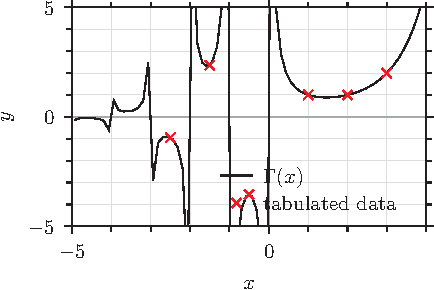
\includegraphics[width=\linewidth]{gamma_pyx.pdf}
	\caption{this is a figure i drew, its pretty}
\end{figure}

\end{document}
